\begin{figure}[tb]
\begin{center}
    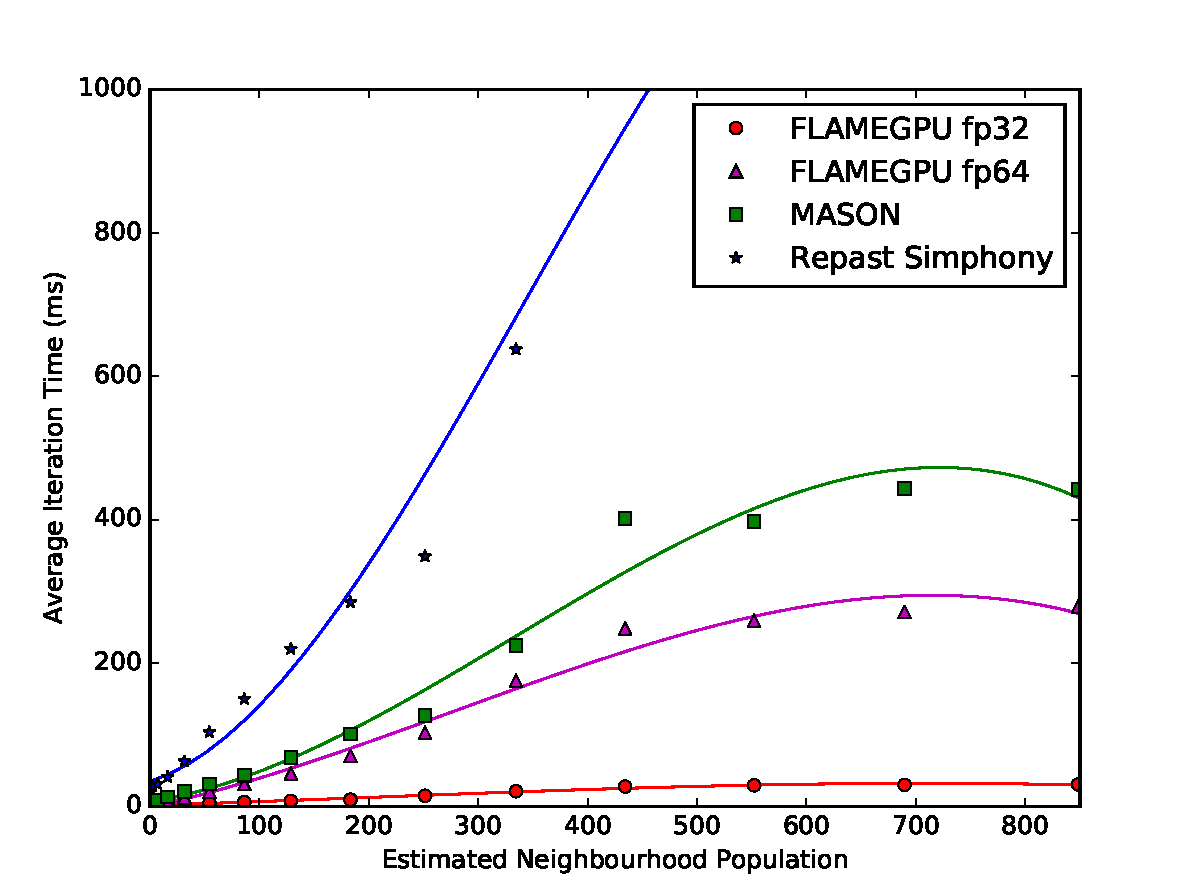
\includegraphics[width=0.7\textwidth]{../resources/problemscale_graph/graph.pdf}
    \caption{\label{fig:graph-agent-pop}The average iteration time of each framework against the agent population.}
\end{center}
%\vspace{-1cm}
\end{figure}
%\vspace{-0.3cm}
\section{Results\label{sec:results}}
%\vspace{-0.4cm}

  Results presented within this section were collected on a single machine running Windows 7 x64 with a Quad core Intel Xeon E3-1230 v3 running at 3.3GHz\footnote{The processor supports hyper-threading, enabling 4 additional concurrent logical threads.}. Additionally the FLAME-GPU framework utilised an Nvidia GeForce GTX 750 Ti \gls{gpu} which has 640 CUDA cores running at 1GHz.
  
  Each of the parameter sets utilised targeted a different performance metric identified in Section \ref{sec:effective-usage}. Results were collected by monitoring the total runtime of 1000 iterations of 3D implementations of the benchmark (executed without visualisation) and are presented as the per iteration mean. Initialisation timings are excluded as the benchmarks focal point is the performance of the near neighbours search carried out within each iteration.
  
  The results in Figure \ref{fig:graph-agent-pop} present the variation in performance as the scale of the problem increases. This is achieved by increasing the parameter $W$, which increases the volume of the environment and hence the agent population. Most apparent from these results is that both the FLAMEGPU implementations, which utilise \gls{gpu} computation as opposed to the other frameworks which utilise a multi-threaded \gls{cpu} approach, consistently outperform the best multi-core framework by a margin which at the largest test-case increases to greater than 6x with 64-bit floating point computation and 10x with the lower precision 32-bit floating point. This is slightly better than the expectations of \gls{gpu} accelerated computation\cite{LK*10}, suggesting their may be further room for optimisation. Although MASON and Repast Simphony are both Java based frameworks, Repast's performance trailed that of MASON by around 3x, investigating this showed Repast's separate operations for updating a particle's spatial and grid locations to be slower than that of MASON which handles both in a single operation. Notably the operation of updating a particles location could not be handled in parallel by MASON or Repast.
  
  The MASON, Repast and 64-bit floating point FLAMEGPU results both have a Pearson correlation coefficient (PCC) \cite{PCC} of 0.99. This is indicative of a linear relationship. Similarly 32-bit floating point FLAMEGPU has a PCC of 0.99 when only agent populations of 100,000 and higher are considered, this suggests that smaller agent populations did not fully utilise the \gls{gpu} during 32-bit floating point computation.
  
  % Width: 50,60..300
  % Density: 0.01
  % Interaction Rad: 5.0
  % Attraction Force: 0.001
  % Repulsion Force: 0.001
  % Iterations: 1000
  \begin{figure}[tb]
\begin{center}
    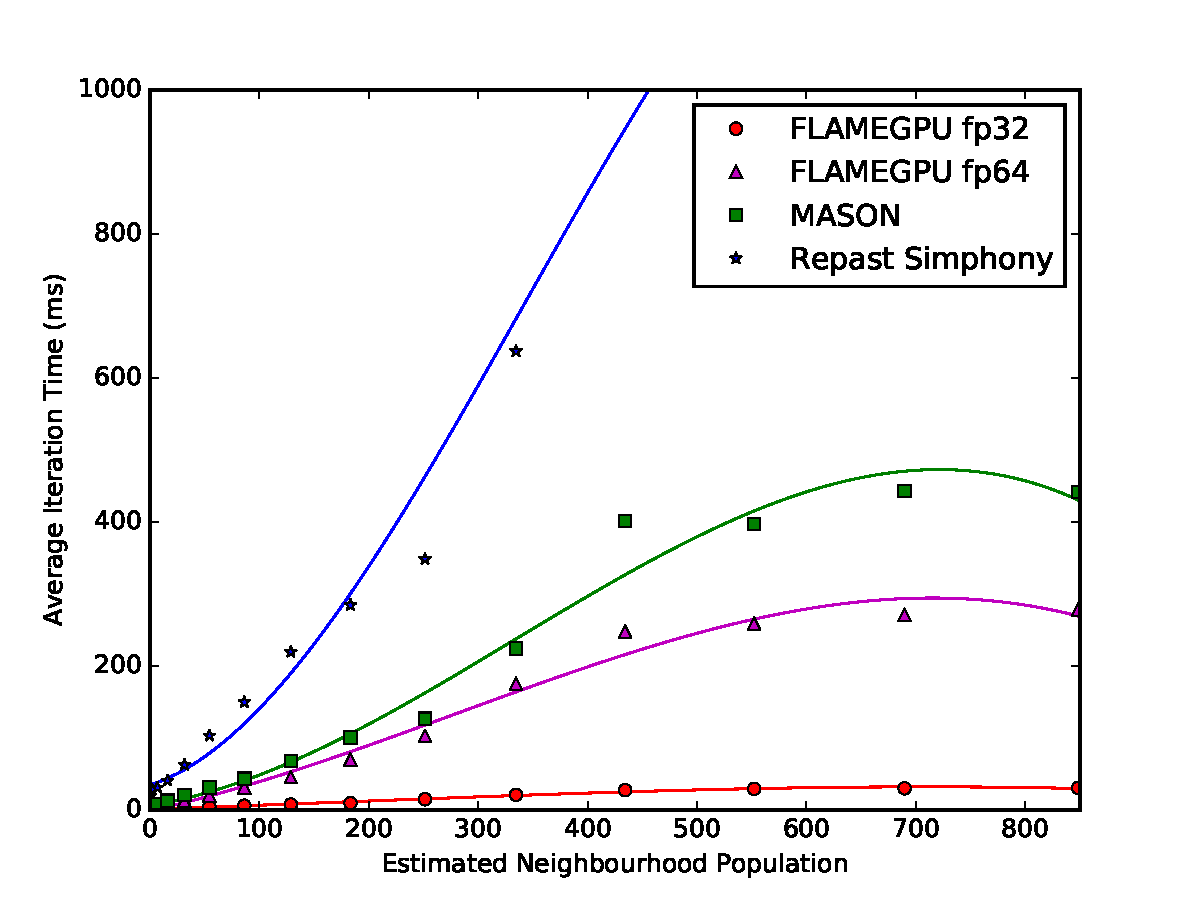
\includegraphics[width=0.7\textwidth]{../resources/neighbourscale_graph/graph.pdf}
    \caption{\label{fig:graph-neighbourhood-pop}The average iteration time of each framework against the estimated neighbourhood population. The estimated neighbourhood population is the calculation of agents within a neighbourhood where agents are uniformly distributed, providing a clearer interpretation of changes to the interaction radius ($r$). }
\end{center}
%\vspace{-1cm}
\end{figure}
  
  The next parameter set, shown in Figure \ref{fig:graph-neighbourhood-pop}, assessed the performance of each framework in response to increases in the agent populations within each neighbourhood. The purpose of this benchmark set was to assess how each framework performed when agents were presented with a greater number of neighbours to survey. This was achieved by increasing the parameter $r$, hence increasing the volume of each agent's radial neighbourhood. All results have a PCC \cite{PCC} of 0.96. This is indicative of a linear relationship, albeit much weaker correlation than that seen within the prior experiment. It is likely that this weaker relationship can be explained by how the agent density becomes more non-uniform as the model progresses, causing the number of agents within each neighbourhood to grow.
  
  % Width: 100
  % Density: 0.01
  % Interaction Rad: 1,2..15
  % Attraction Force: 0.001
  % Repulsion Force: 0.001
  % Iterations: 1000
  The final parameter set assessed variation in performance in response to increased entropy. This is was achieved by adjusting the parameters $k_{att}$ and $k_{rep}$, causing the force exerted on the agents to increase, subsequently causing them to move faster.
  
  The purpose of this benchmark was to assess whether any of the frameworks benefited from reduced numbers of agents transitioning between spatial partitions. The results however showed no substantial relationship between increased particle speed and performance.
  % Width: 50,60..300
  % Density: 0.01
  % Interaction Rad: 5.0
  % Attraction Force: 0.001
  % Repulsion Force: 0.001
  % Iterations: 100